\documentclass{ximera}

\begin{document}
\begin{problem}
  Two numbers, $x$ and $y$, are shown below on a number line.
  \begin{image}
    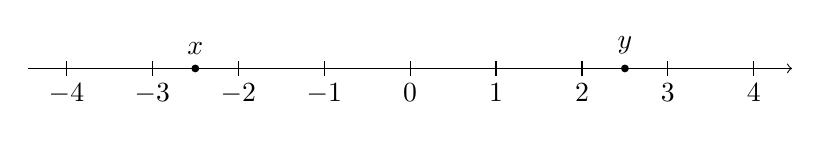
\begin{tikzpicture}[x=0.09\textwidth]
      \draw[-{>[scale=1.75]}] (-0.4\textwidth,0) -- (0.4\textwidth,0);
      \foreach \x in {-4,...,4} {%
        \draw (\x,-.1) -- (\x,.1);
        \node[anchor=north,yshift=-2pt] at (\x,0) {$\x$};
      }
      \draw (-2.5,0) node [circle,fill,inner sep=1pt,label=above:$x$](e){};
      \draw (2.5,0) node [circle,fill,inner sep=1pt,label=above:$y$](e){};
    \end{tikzpicture}
  \end{image}
  Which is closest to $xy$?
  \begin{multipleChoice}
    \choice[correct]{$-6.25$}
    \choice{$-4.75$}
    \choice{$4.75$}
    \choice{$6.25$}
  \end{multipleChoice}
\end{problem}
\end{document}
